The model was implemented on a mesoscale mouse connectome, which organized the mouse brain into 13 cortices, made up of 213 subcortices total and measured the connection strengths between the subcortices \cite{Oh2014}.
These connection strengths were then reduced to those with sufficient certainty ($p < 0.01$), and segmented as follows:
\begin{equation}
  \label{eq:mouse_segmentation}
  G_{j k}
  =
  \begin{cases}
    0, & \text{if } O_{j k} < 10^{-4} \\
    1, & \text{if } O_{j k} < 10^{-2} \\
    2, & \text{if } O_{j k} < 1 \\
    3, & \text{otherwise}
  \end{cases}
\end{equation}
where $O_{j k}$ is the raw connection strength provided by \cite{Oh2014}.
$G$ is shown in \cref{fig:mouse_connectome}, and is shown broken down into its inter- and intra-connections in \cref{fig:network_breakdown}.
A useful aspect of this brain network is that the standard graph whose topology it most resembles is a small-world or Watts-Strogatz graph \cite{Oh2014}.
This graph topology lends itself well to the development of chimera states, as it facilitates nonlocal coupling \cite{Hizanidis2016}.

\begin{figure}[ht]
  \centering
  \begin{subfigure}{0.45\textwidth}
    \centering
    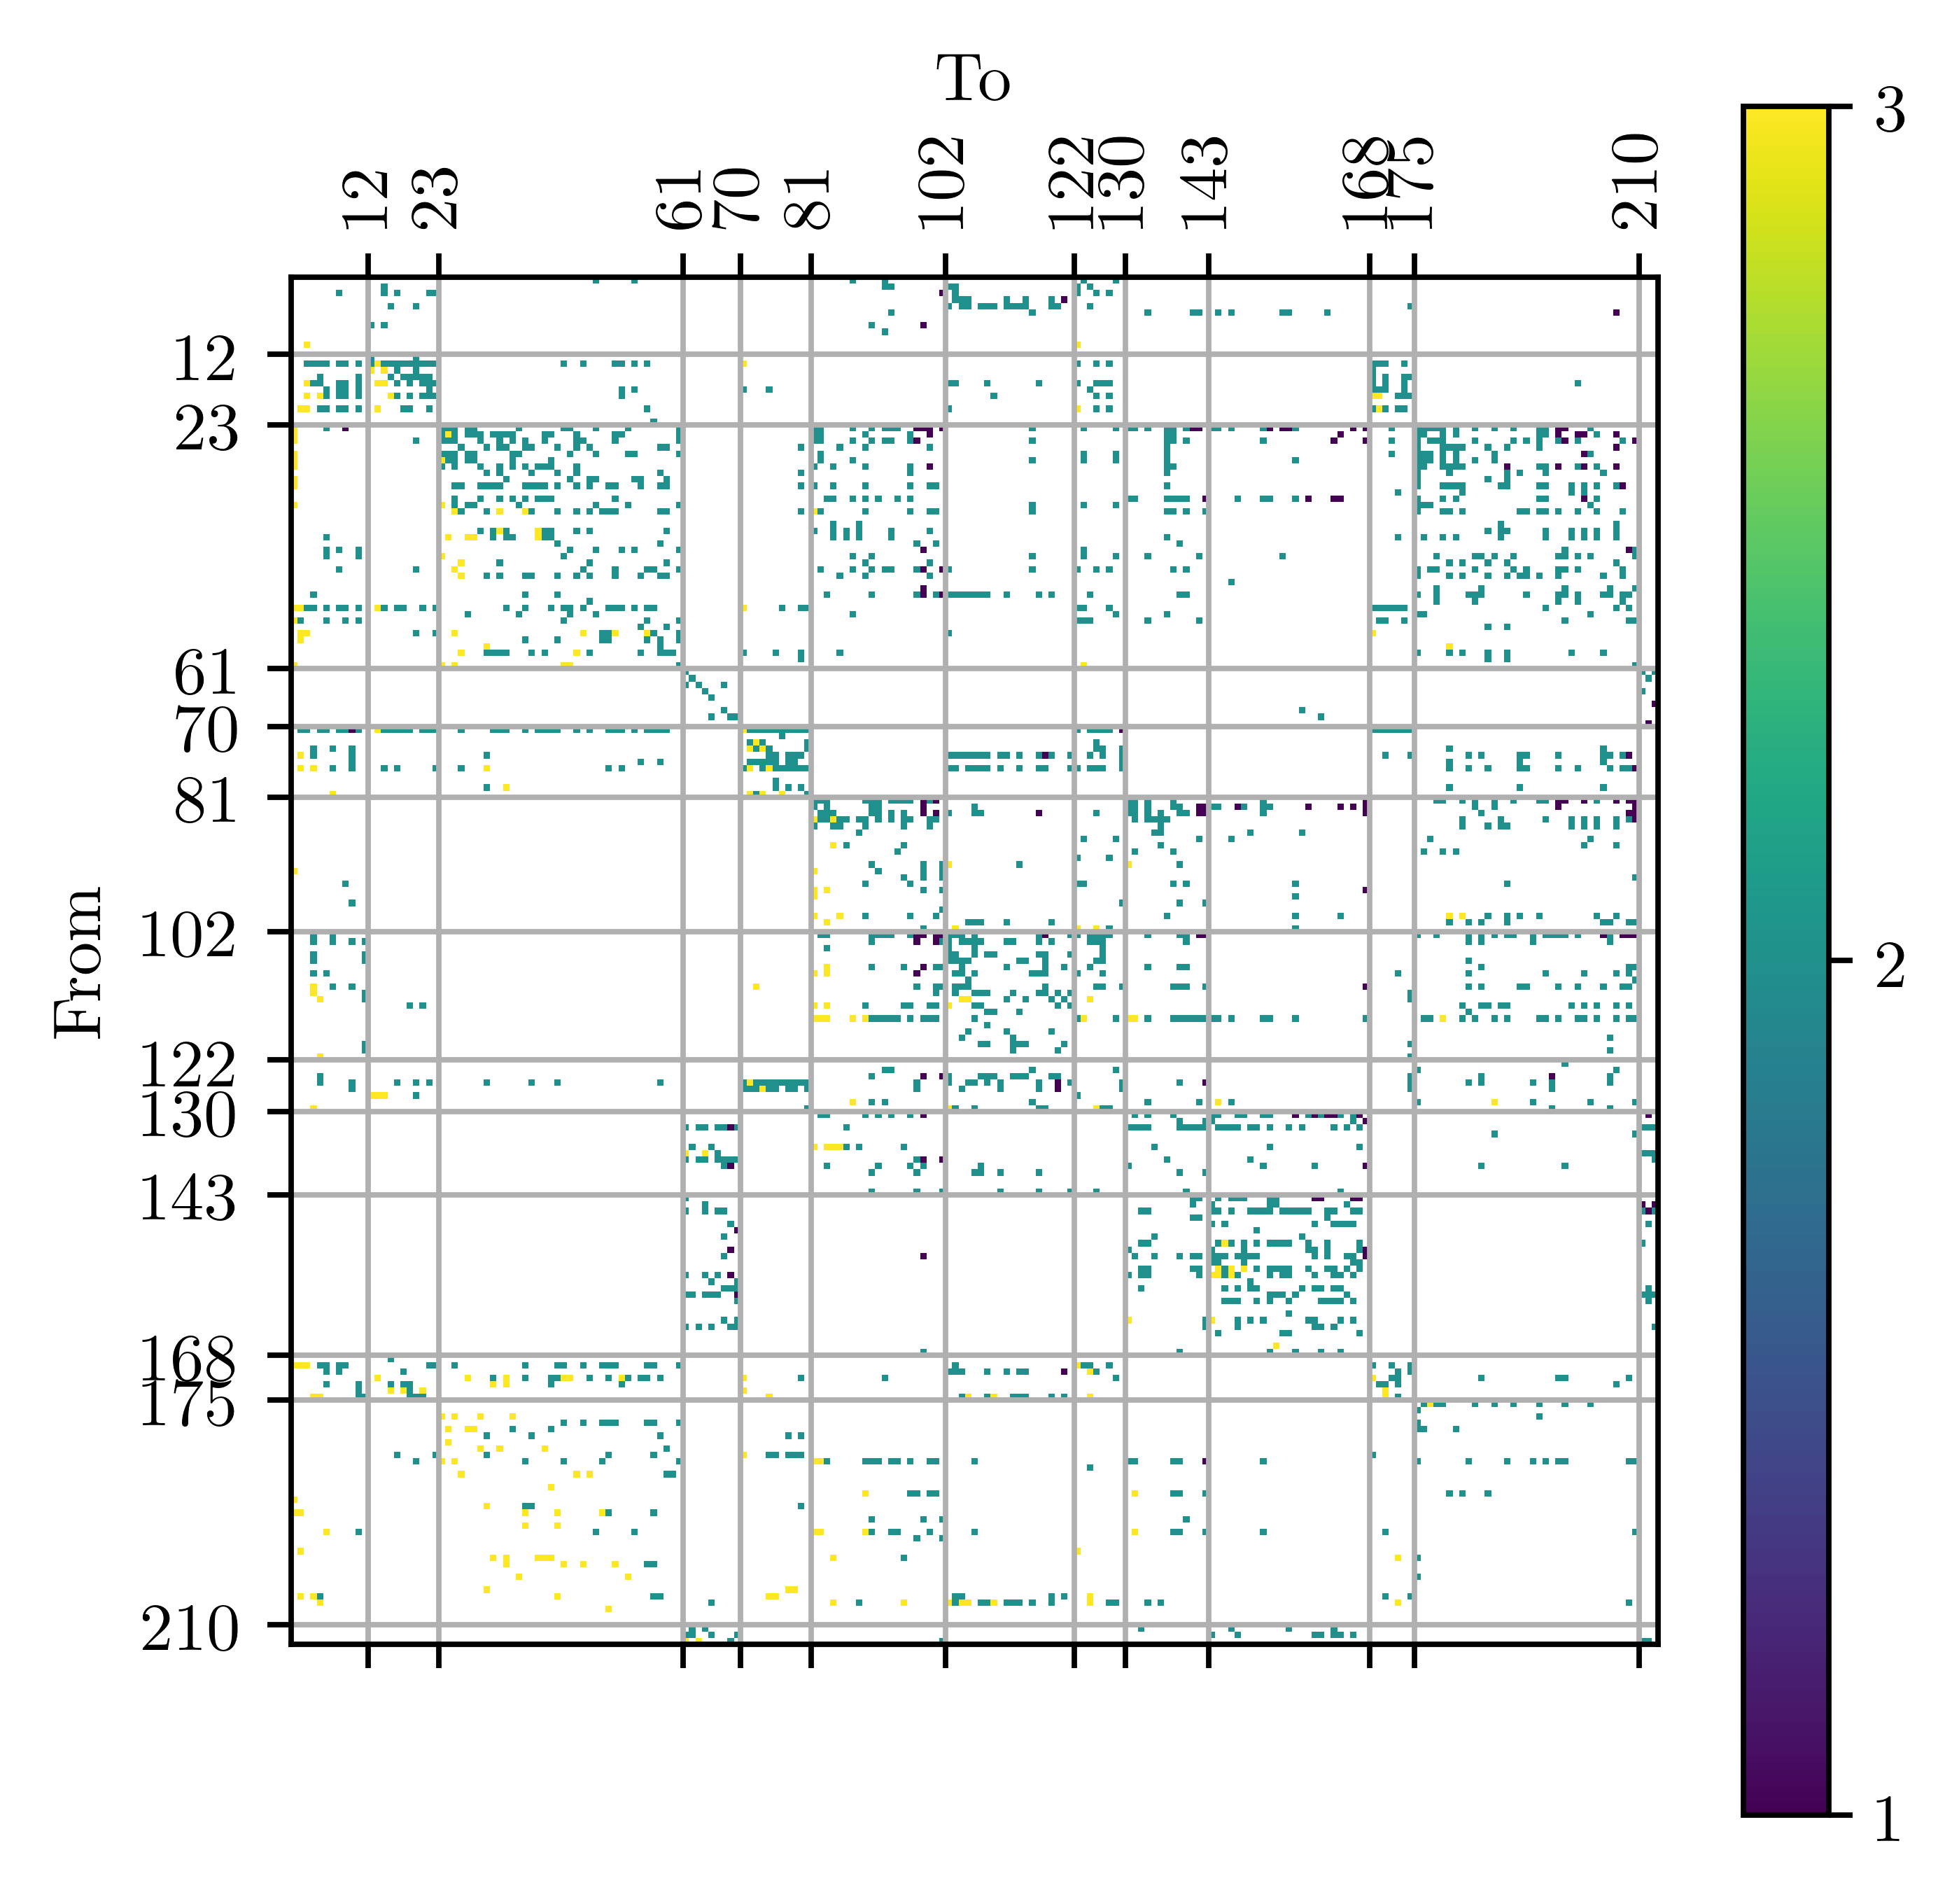
\includegraphics[width=\textwidth]{figure/n}
    \caption{Matrix representation}
    \label{fig:mouse_matrix}
  \end{subfigure} %
  \begin{subfigure}{0.45\textwidth}
    \centering
    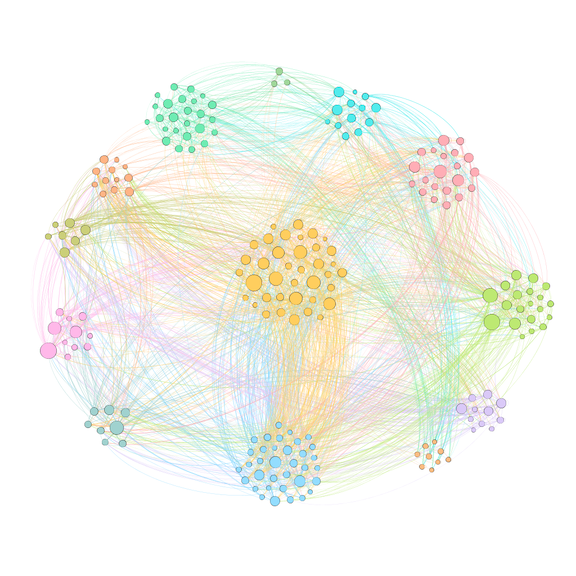
\includegraphics[width=\textwidth]{figure/network}
    \caption{Embedding}
    \label{fig:mouse_embedding}
  \end{subfigure}
  \caption[Mouse connectome]{(a) A matrix representation of the mouse connectome, with strengths as defined by \cref{eq:mouse_segmentation}.
    The cortices represented are, left to right (top to bottom),
    the striatum,
    the olfactory areas,
    the isocortex,
    the crebellar cortex,
    the hippocampal formation,
    the midbrain,
    the hypothalamus,
    the pallidum,
    the pons,
    the medulla,
    the cortical subplate,
    the thalamus,
    and the cerebellar nuclei.
    (b) An embedding of the graph.
    Edge colors indicate the source location.
  }
  \label{fig:mouse_connectome}
\end{figure}

Another benefit to this network is that it is accurate and complete.
Given the complexity of brains, creating an accurate structural or functional connectome is extremely difficult.
It has yet to be done to a large-scale extent in humans, and was only recently done in mice.
Additionally, as mice are common analogues for humans in laboratory settings, the mouse seemed a fitting ``guinea pig'' for the creation of chimera states.

\begin{figure}[ht]
  \centering
  \begin{subfigure}{0.45\textwidth}
    \centering
    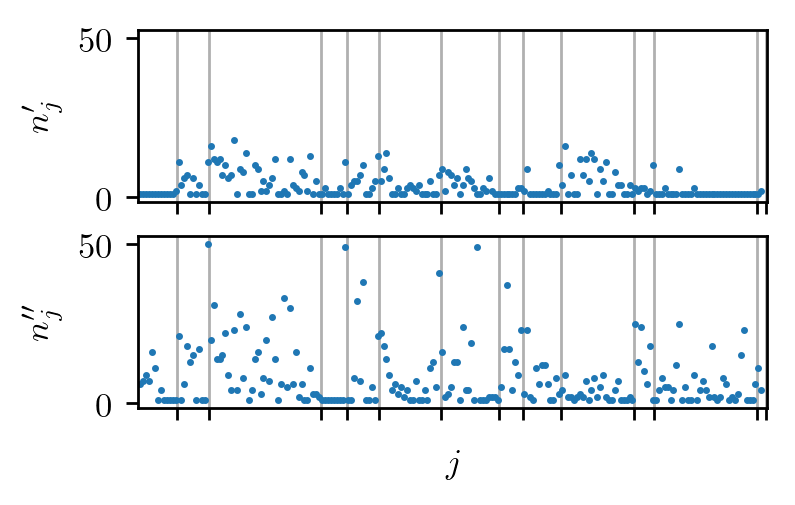
\includegraphics[width=\textwidth]{figure/n_prime}
    \caption{$n'$ and $n''$}
    \label{fig:n_prime}
  \end{subfigure} %
  \begin{subfigure}{0.45\textwidth}
    \centering
    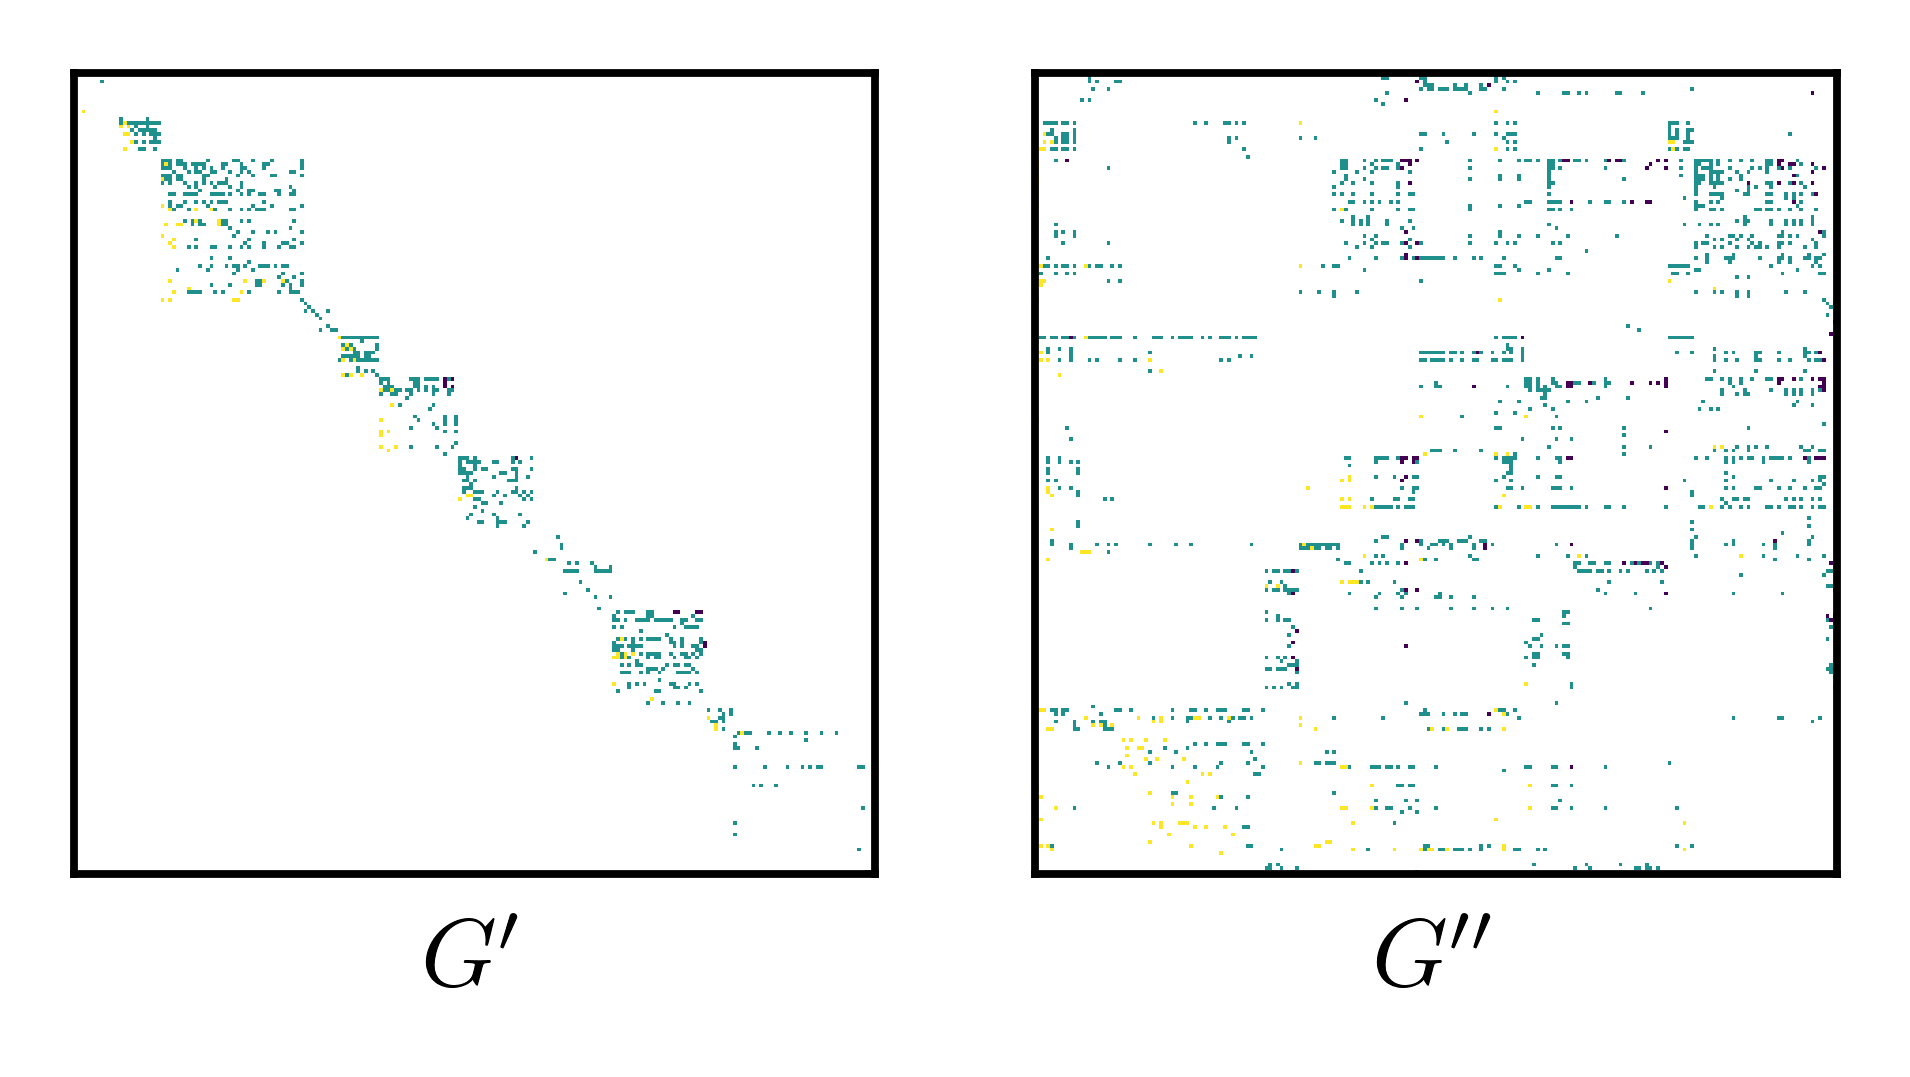
\includegraphics[width=\textwidth]{figure/g_prime}
    \caption{$G'$ and $G''$}
    \label{fig:g_prime}
  \end{subfigure}
  \caption[Network breakdown]{A breakdown of the network.
    (a) shows $n_{j}'$ and $n_{j}''$, effectively the number of nonzero elements in the $j$th row of $G'$ and $G''$, respectively.
    (b) shows $G'$ and $G''$, which are $G$ (\cref{fig:mouse_matrix}) only within and between cortices, respectively.
  }
  \label{fig:network_breakdown}
\end{figure}

\begin{figure}[ht]
  \centering
  \begin{subfigure}{0.45\textwidth}
    \centering
    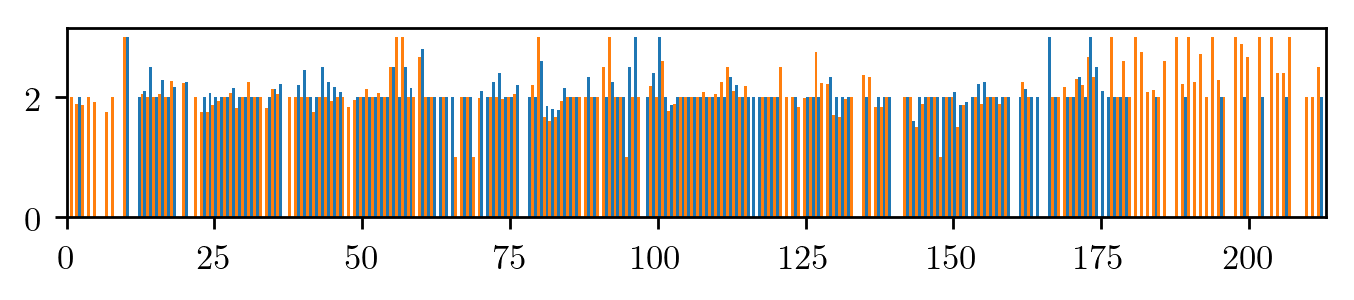
\includegraphics[width=\textwidth]{figure/g_over_n}
    \caption{All values}
    \label{fig:g_over_n}
  \end{subfigure} %
  \begin{subfigure}{0.45\textwidth}
    \centering
    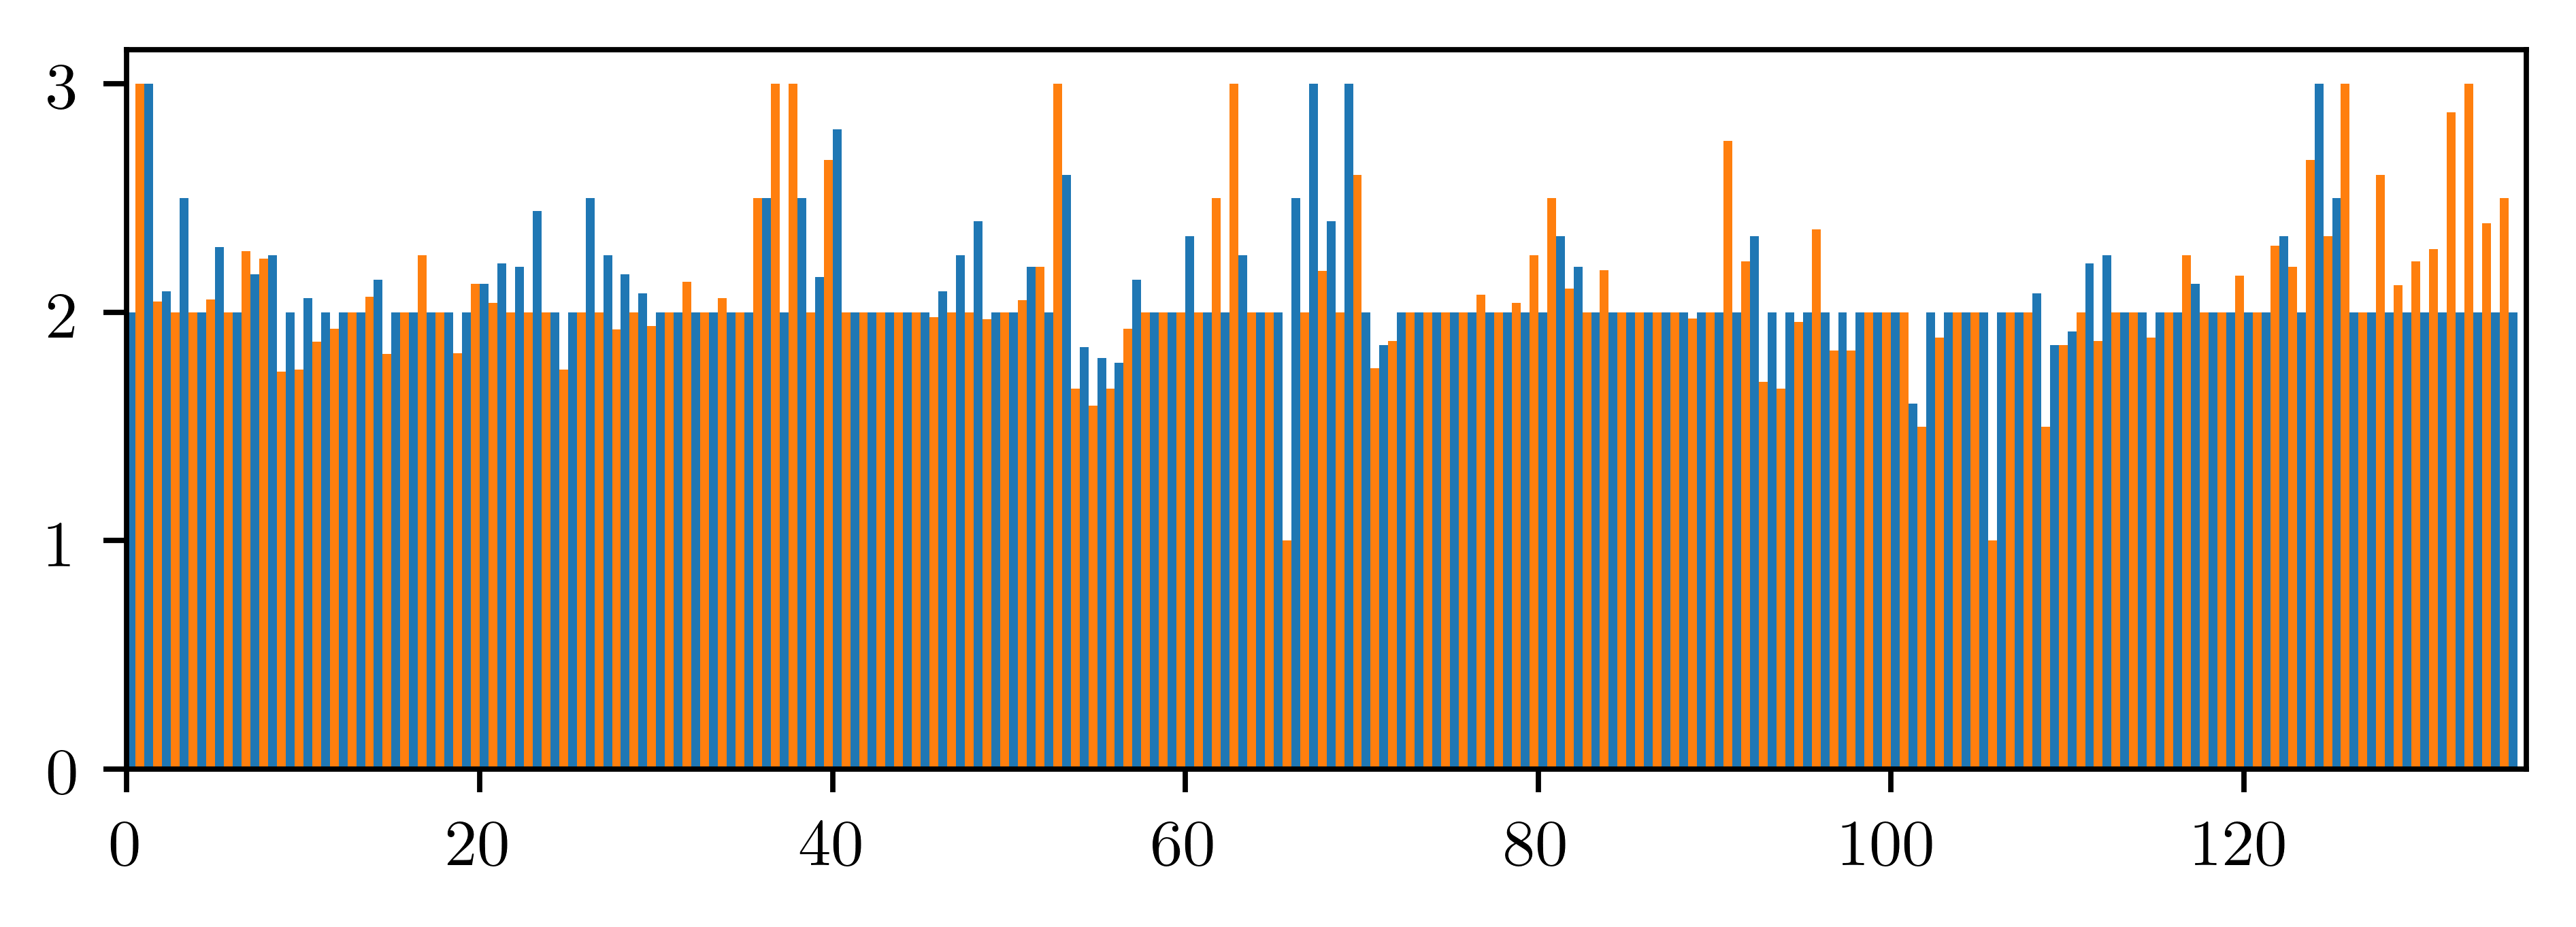
\includegraphics[width=\textwidth]{figure/g_over_n_drop}
    \caption{Dropped zeros}
    \label{fig:g_over_n_drop}
  \end{subfigure}
  \caption[Average strengths]{The average connection strengths for each neuron $j$, within cortices (blue) and between them (orange).
    (a) All of the subcortices.
    (b) All of the subcortices for which neither intra- nor inter-cortical average strength was 0.
  }
  \label{fig:average_strengths}
\end{figure}

%%% Local Variables:
%%% mode: latex
%%% TeX-master: "../../main"
%%% End:
